\documentclass{article}
\usepackage{geometry}
\geometry{a4paper, margin=1.2in}
\setlength{\parskip}{0.5em}
\usepackage{graphicx}
\usepackage[utf8]{inputenc}
\usepackage{amsmath}
\usepackage{float}
\title{\textbf{Jamie Vardy}}
\author{Atharv Singh Patlan}
\date{\today}

\begin{document}

\maketitle
\textbf{Jamie Richard Vardy} is an English footballer who plays as a striker for Premier League club \textbf{Leicester City}. He joined Leicester City in 2012 when they were a second division team, and helped greatly in their promotion to the premier league in the 2014/15 season. Here we have a look at his performance across the previous 6 seasons and compare him with the current PL greats!

One of the best ways to identify the breakaway season for any attacking player in the FPL world is to have a look at the amount of \textbf{change in the player's cost in FPL} (the cost they need to play to include the player in the team). A higher cost at the end of the season means the player has gained popularity due to his performance over the season.
\begin{figure}[H]
    \centering
    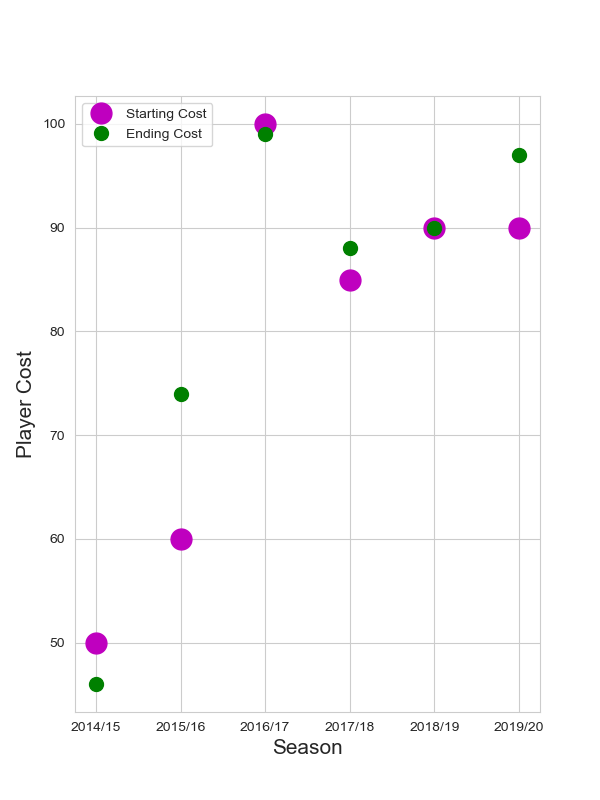
\includegraphics[width=0.6\linewidth]{assets/cost_season.png}
    \caption{Jamie Vardy's initial and final cost comparison over the seasons}
    \label{fig:cost_season}
\end{figure}

Figure \ref{fig:cost_season} clearly demarcated \textbf{2015/16 as the breakaway season} for Vardy. There was a marked \textbf{increase} in his cost over the season, from a measly cost of \textbf{60, to 74}. The high increase in his cost over the season also raised the expectations in the minds of FPL players about him, leading to an astounding increase in his initial cost in the 2016/17 to 100, a jump of 40 over the previous season!

However, Vardy is \textbf{not} a one-season man! He has been a \textbf{consistent performer} for the Leicester team, scoring goals and raking assists for them across the seasons.

\begin{figure}[H]
    \centering
    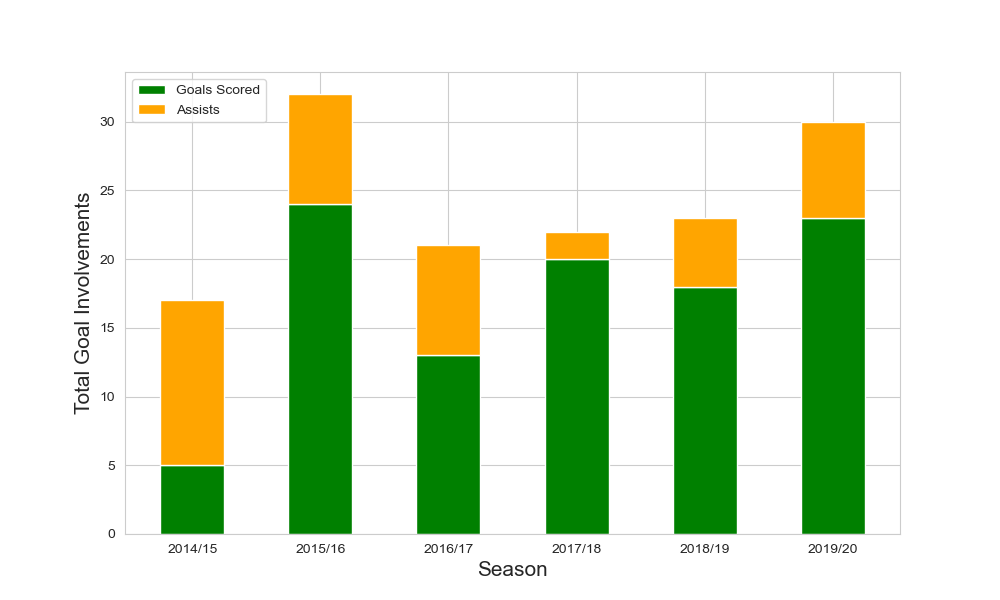
\includegraphics[width=1\linewidth]{assets/goalinvolv_season.png}
    \caption{Vardy: Goal Involvements over the seasons}
    \label{fig:goalinvolv_season}
\end{figure}
It can be seen from Figure \ref{fig:goalinvolv_season} that Vardy has directly contributed in \textbf{more than 20 goals every season since 2015/16}, even after a couple of tumultuous seasons for Leicester, 2016/17 and 2017/18 with the sacking of their PL winning boss Claudio Ranieri.

\begin{figure}[H]
    \centering
    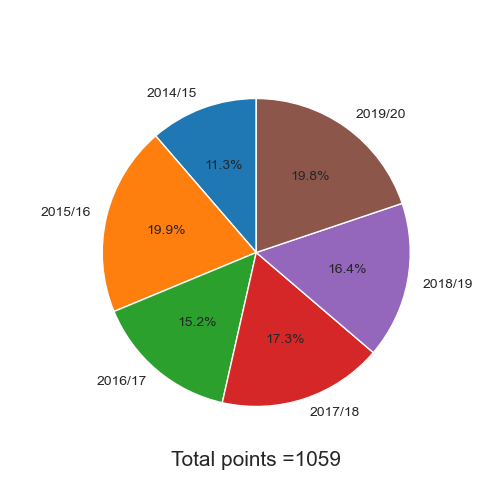
\includegraphics[width=0.5\linewidth]{assets/points_season.png}
    \caption{Vardy: Percentage of Total points accumulated over the seasons}
    \label{fig:points}
\end{figure}

Figure \ref{fig:points} shows the \textbf{trust} FPL players have in Vardy, as he claimed \textbf{more than 15\%} of his total points in the 2016/17 season, a season where his form had greatly dipped.

His \textbf{proficiency as a striker} can be seen on the pitch with his \textbf{excellent fitness levels} and \textbf{efficiency on the pitch}. However, he is not one to bask in his glory and sit back. He continuously works to \textbf{improve himself and his gameplay}.
\begin{figure}[H]
    \centering
    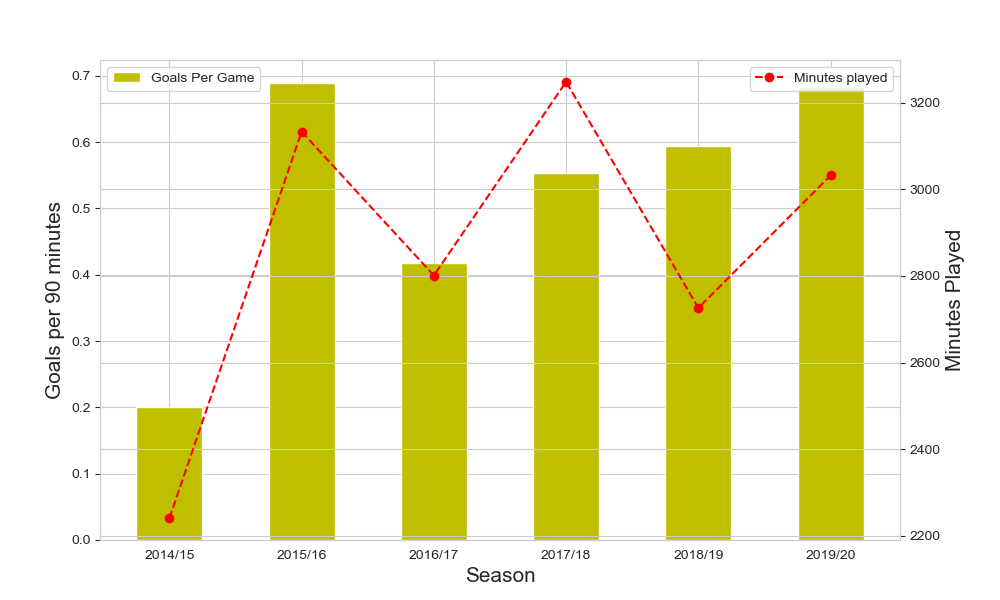
\includegraphics[width=1\linewidth]{assets/gpm_season.png}
    \caption{Vardy: Goals Per Match and Minutes Played over the seasons}
    \label{fig:gpm_season}
\end{figure}
He has \textbf{consistently} played more than \textbf{2700 minutes} every season since his Premier League Debut. His immense focus on his training and skills can be seen by the \textbf{ever-increasing} Goals Per Match rate he has had since the 2016/17 season, to come at a scoring rate at par with his glorious season of 2015/16, at around \textbf{0.7}.

However, in order to see his actual talents, it is necessary to compare him with the current best players at his position in the Premier League. We compare Vardy's FPL Value across the seasons with those of the top scorers of the league in the 2019/20 season, which is the most important criteria FPL players consider while chosing a player, with a value above 2 being a symbol of excellence.

His \textbf{excellent performance} is revealed again in Figure \ref{fig:value_season_all}. It can be seen that Vardy has received a \textbf{value close to 2 in 5 of the previous 6 seasons}. None of the other top players this season have this statistic.

\begin{figure}[H]
    \centering
    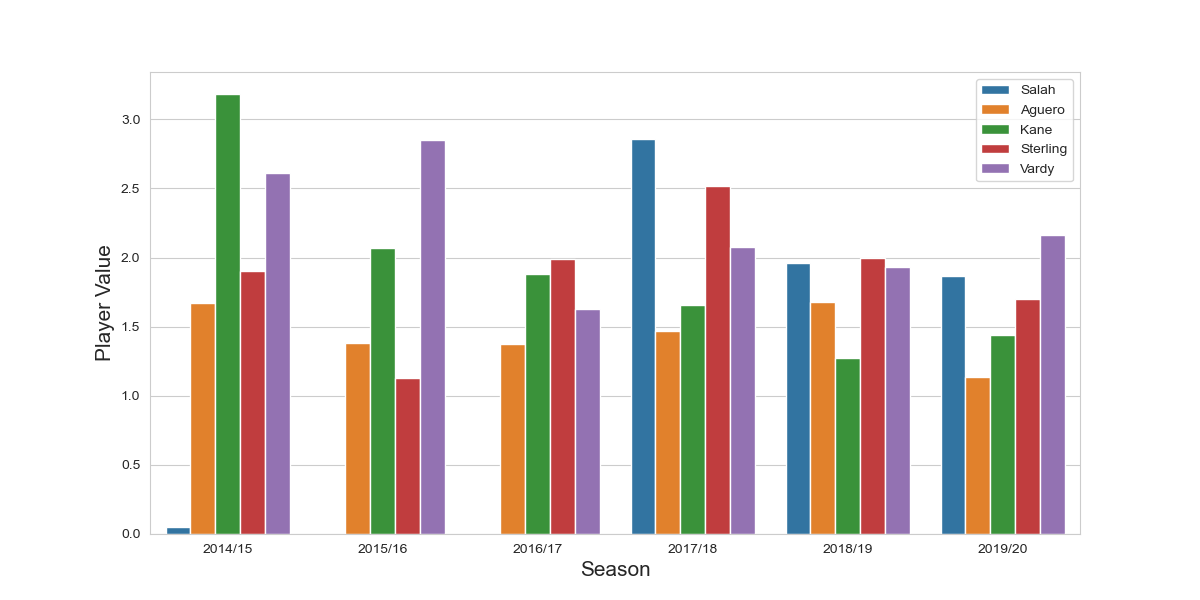
\includegraphics[width=1\linewidth]{assets/value_season_all.png}
    \caption{Vardy: Comparison of Value over the seasons with top players}
    \label{fig:value_season_all}
\end{figure}

I end this report with the real juice and the thing the real EPL (not the FPL) fans were looking for! The goal scoring statistics! Here, I leave Figure \ref{fig:goal_season_all} for you to savour and enjoy!

\begin{figure}[H]
    \centering
    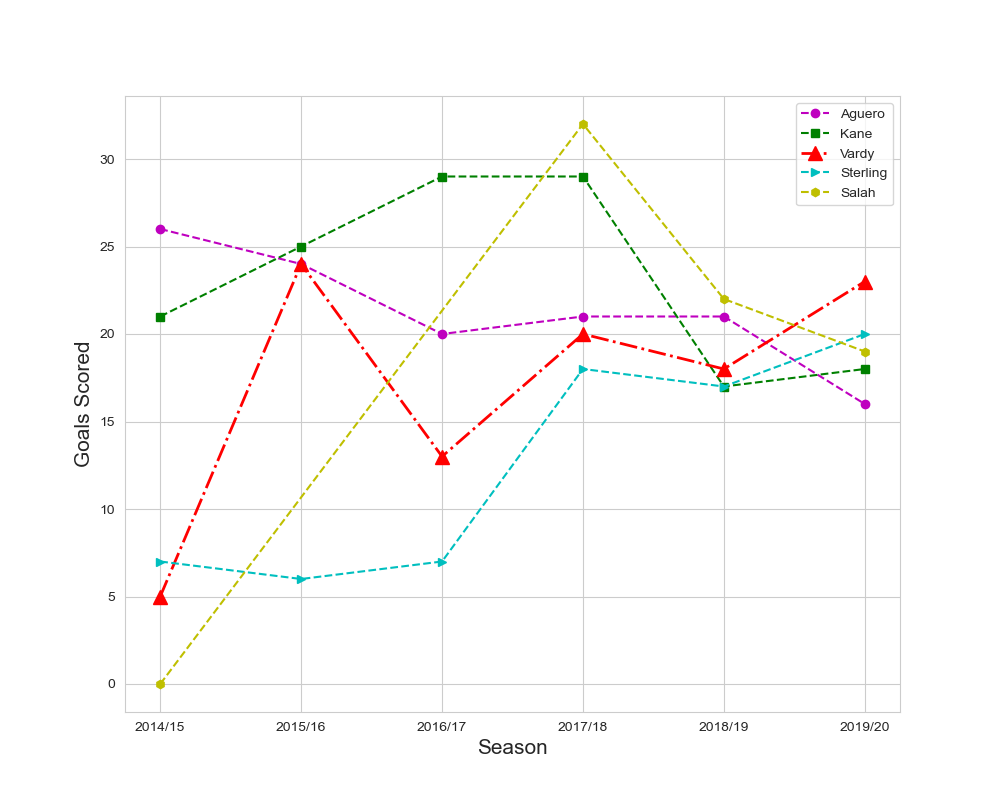
\includegraphics[width=0.95\linewidth]{assets/goal_season_all.png}
    \caption{Vardy: Comparison of goal scoring record over the seasons with top goal-scorers}
    \label{fig:goal_season_all}
\end{figure}
\end{document}
